\documentclass[11pt, a4paper,twocolumn]{jarticle}
\usepackage[dvipdfmx]{graphicx}
\usepackage{listings,jlisting}
\usepackage{docmute}
\begin{document}
\begin{titlepage}
  \begin{center}
    {\Huge F 光と制御}\\
    \vspace{30truept}
    {\huge   提出者 : 08A17153 羽田充宏}\\ % 学籍番号
    {\huge 共同実験者 : 08A17179 牧野将之}\\
    {\huge       : 08A17205 森本拓実}\\ % 学籍番号
    \vspace{50truept}

    \begin{list}{}{\setlength{\leftmargin}{95pt}}
    \item {\huge 実験実施日 : 2019年10月7日}\\
    \vspace{10truept}
    \item {\huge 実験実施日 : 2019年10月21日}\\
    \vspace{10truept}
    \item {\huge 実験実施日 : 2019年10月28日}\\
    \vspace{10truept}
    \item {\huge 実験実施日 : 2019年11月11日}\\
    \vspace{10truept}
    \item {\huge 実験実施日 : 2019年11月25日}\\
    \vspace{10truept}
    \item {\huge 実験実施日 : 2019年11月25日}\\
    \vspace{40truept}

    \end{list}
    \vspace{50truept}

  \end{center}
\end{titlepage}


% template======================================================
% \section{}
% \subsection{}
% \subsubsection{Purpose}
% \subsection{Equipment}
% \begin{itemize}
%     \item
% \end{itemize}
% \subsubsection{Procedure}
% \subsubsection{Result}
% \subsubsection{Discussion}
%=============================================================
% \begin{figure}[ht]
%  \begin{center}
%   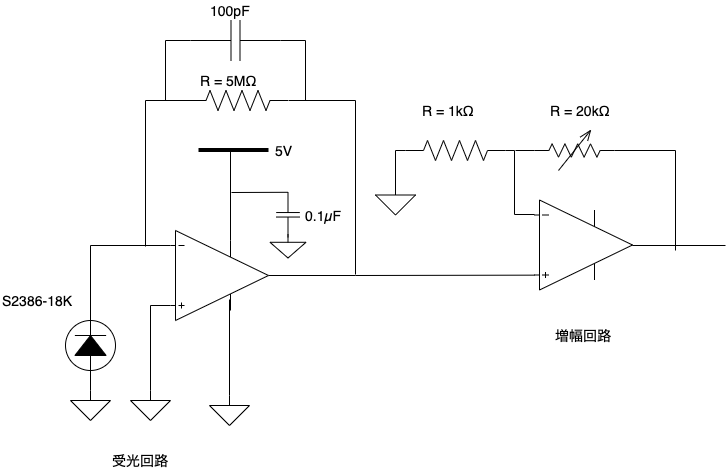
\includegraphics[width=0.8\linewidth]{fig1.png}
%  \end{center}
%  \caption{74HC14}
%  \label{fig:1}
% \end{figure}
% \clearpage
%=============================================================
\twocolumn
[
\begin{center}
    \textbf{\Large 実験概要}\\
    \begin{flushleft}
        様々な光応用分野で用いられている光走査技術の原理を理解し,その実現に必要となる要素技術(半導体レーザー制御,受光回路動作,モーター駆動,走査系構築,コンピュータ制御)を修得する.さらに,具体的な光応用システムとして(一次元)画像スキャナを構成する.画像データの取り込みにおける様々な特性を測定し,システムとしての性能を評価,議論する.
    \end{flushleft}
\end{center}
\vspace{30truept}
]
%=============================================================
\documentclass[11pt, a4paper,twocolumn]{jarticle}
\usepackage[dvipdfmx]{graphicx}
\usepackage{listings,jlisting}

\begin{document}
%=============================================================
\section{受光回路の作成}
\subsection{目的}
走査計測に必要となる受光回路を作成する.
また,今回作成する受光回路は最終日まで使用する.
\subsection{手順}
半田ごてを用いて図に示すように受光回路の作成を行った.
この時受光回路のプリント基板を金属の作業台にそのまま置いてショートさせないように注意した.

\begin{figure}[ht]
 \begin{center}
  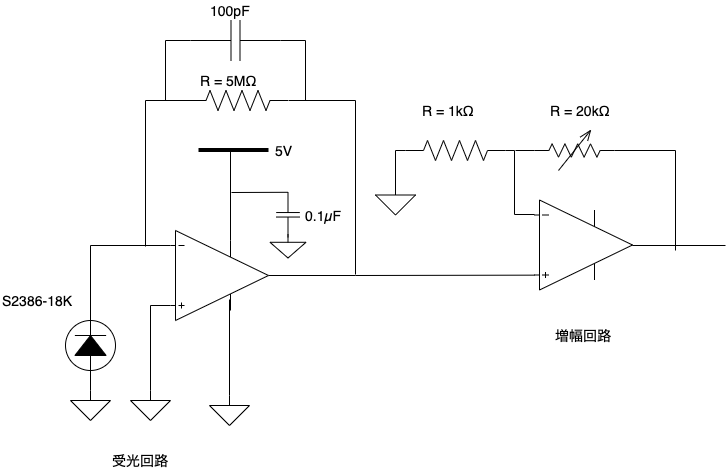
\includegraphics[width=0.8\linewidth]{fig1.png}
 \end{center}
 \caption{受光回路}
 \label{fig:1}
\end{figure}

\subsection{結果}
フォトダイオードに蛍光灯の光を入射させ,手で覆い隠す操作を繰り返しオシロスコープで出力電圧を確認したところ手で覆い隠すと出力電圧は0付近になり,手をどけると60Hz付近の周波数の出力波が観測された.
また可変抵抗${R_2}$を調節することで受光回路の感度を調節できることを確認できた.

\subsection{考察}
手で覆うことで出力が0付近になり,手をどかすことで出力電圧を観測できたことから受光回路は正常に機能していると考えられる.
また手をどかした際に60Hz付近の出力電圧を観測したのは蛍光灯などの教室内の電化製品から発せられる電磁波が観測されたためであると考えられる.
これは西日本の交流電流の周波数が60Hzであることに一致する.
%=============================================================
\newpage
\end{document}

\documentclass[11pt, a4paper,twocolumn]{jarticle}
\usepackage[dvipdfmx]{graphicx}
\usepackage{listings,jlisting}

\begin{document}
%=============================================================
\section{半導体レーザーの発光特性}
\subsection{目的}
この実験の目的は,外部信号により発光パワー変調が可能である半導体レーザーの制御である.
今回は前セメスターのデジタル計測実験でのAD/DAデバイスを用いてパソコンでのプログラムを介してのレーザー制御を行う.
\subsection{手順}
半導体レーザーの赤色導線,黒色導線をそれぞれ電源の5V,GNDに接続し白色導線をAD/DAデバイスに接続した.
キーボード入力により信号電圧(0-5V)を制御するプログラムを記述した.
この時のプログラムはデジタル計測の実験での電圧出力プログラムに定電圧を出力できるように手を加えて流用した.
次に半導体レーザーの前方にパワーメーターを配置し,半導体レーザーの出力を変えながら光パワーを測定した.
また,パワーメータの代わりに前回の実験で作成した受光回路を用いてオシロスコープにて出力電圧を計測した.
さらに,測定した結果をグラフに書き込んだ.
この時受光回路を予め一番強いレーザー光を入射した際に5Vに達して飽和しないように可変抵抗により感度を調節しておいた.

\subsection{結果}
パワーメーター,受光回路で測定した結果は以下のようになった.
ここでパワーメータでは単位はW,受光回路では単位はVのことに注意する.
グラフよりどちらの測定においてもレーザーへの入力電圧が1.2V付近から測定値の増加は緩やかになり飽和していることが読み取れる.
また,パワーメータの飽和点は1.165Vであったのに対し受光回路の飽和点は1.7Vであった.
さらに,パワーメータでの測定ではレーザー出力は0.83Vで初めて検出されたのに対し,受光回路での測定ではレーザー出力は1.05Vで初めて観測された.

\begin{figure}[ht]
 \begin{center}
  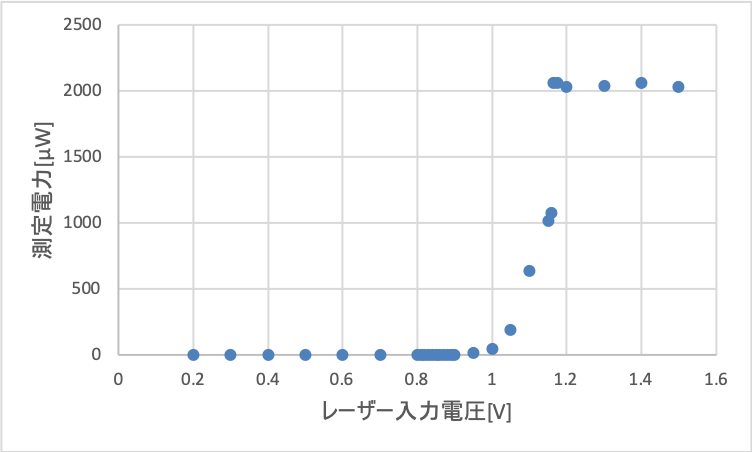
\includegraphics[width=0.8\linewidth]{fig2.png}
 \end{center}
 \caption{パワーメータ測定}
 \label{fig:2}
\end{figure}

\begin{figure}[ht]
 \begin{center}
  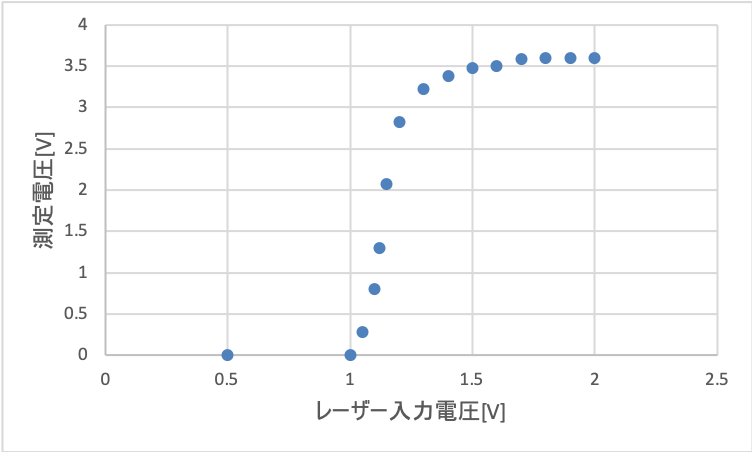
\includegraphics[width=0.8\linewidth]{fig3.png}
 \end{center}
 \caption{受光回路測定}
 \label{fig:3}
\end{figure}

\subsection{考察}
まず二つの測定結果より半導体レーザーが発光するにはある程度の電圧を入力する必要があり,その閾値は1V付近であると考えられる.
またパワーメータと受光回路で初めてレーザー出力が観測される値が異なるのはパワーメータの測定実験後に半導体レーザーのレンズを取り外してしまったため,結果として半導体レーザーの広がり角が大きくなり測定されるまでにより大きな入力電圧を要する必要があったためと考えられる.
さらに受光回路において光パワーを線形的に測定できる範囲はグラフより1.0~1.2Vであると考えられる.

%=============================================================
\newpage
\end{document}

\documentclass[11pt, a4paper,twocolumn]{jarticle}
\usepackage[dvipdfmx]{graphicx}
\usepackage{listings,jlisting}

\begin{document}
%=============================================================
\section{光信号の取り込み系の作制}
\subsection{目的}
この実験では最終的な実験光学系の可動ミラーを除いた光学系を作成することにより一点の光信号を取り込むことを可能にすることが目的である.

\subsection{手順}
図\ref{fig:a}のように光学系を組み立てた.
まず,半導体レーザーを焦点距離40mmの凸レンズを用いて平行光にしてからハーフミラーを通過させ,焦点距離100mmの凸レンズによって集光させた.
今度は入力物体から発せられる点光源が逆の光路を辿ることによりコリメートされた光がハーフミラーで反射され,焦点距離40mmの凸レンズを用いることでフォトダイオードの感光素子に集光されるようにした.
またフォトディテクターから得られた電圧をパソコンにテキストファイルとして書き込むプログラムを作成した.
このプログラムも前セメスターで行ったデジタル計測のプログラムを流用して使った.

\begin{figure}[ht]
 \begin{center}
  \includegraphics[width=0.8\linewidth]{fig4.png}
 \end{center}
 \caption{光取り込み系の動作確認のための光学系}
 \label{fig:a}
\end{figure}

\subsection{結果}
初めの週の実験では黒い紙と白い紙を交互に入力してもフォトダイオードからの電圧差を観測することができなかった.
二週間目の実験では紙の色に応じてフォトダイオードの出力電圧が変わることが確認できた.

\subsection{考察}
まず,初めの実験で入力物体に応じた電圧差を観測できなかった理由はビームエキスパンダーを作った際にうまくコリメートできていなかったために集光スポットが大きくなってしまったからだと考えられる.
次に半導体レーザーの方位角の設定について考える.
半導体レーザーは方位角によって発散角が異なっており楕円形のビーム広がりを持つ.
後の実験においては縦縞の周期的な光信号を読み取ることが目的なので回折限界の式(一次元走査光学系の特性評価)より平行光の直径が大きいほど集光スポットは小さくなる.
従って今後の実験においては楕円の長軸を水平にした状態でレーザーを設置することが望ましいと考えられる.


%=============================================================
\newpage
\end{document}

\documentclass[11pt, a4paper,twocolumn]{jarticle}
\usepackage[dvipdfmx]{graphicx}
\usepackage{listings,jlisting}

\begin{document}
%=============================================================
\section{定常状態での光信号の取り込み}
\subsection{目的}
この実験では定常状態(走査しない状態)での入力物体と取得信号の関係について検証する.

\subsection{手順}
図\ref{fig:5}のような光学濃度の異なる物体の中心に対して得られる信号を測定した.
次に物体のエッジに対して得られる信号を測定した.
ここで左上のサンプルから光学濃度の大きい順に1,2,...,11とラベリングすることにした.
また今回の測定はデータ数100点として測定を行いそのデータの平均を求めた.
\begin{figure}[ht]
 \begin{center}
  \includegraphics[width=0.8\linewidth]{fig5.png}
 \end{center}
 \caption{サンプル}
 \label{fig:5}
\end{figure}

\subsection{結果}
測定の結果中心に対しての光強度は表\ref{fig:hoge}のようになった.
またエッジ周辺の光信号の取り込みにおいてはエッジに集光スポット(測定点)が乗った時にサンプル番号1と同じ電圧が得られ,集光スポットがエッジから外れるとそのサンプルの中心と同じ電圧が得られた.

\begin{table}[ht]
\centering
\caption{光信号の取り込み}
\label{my-label}
\begin{tabular}{c c}
\hline
サンプル番号 & 測定電圧[V] \\ \hline
1 & 0.594286267 \\
2 & 0.684387733 \\
3 & 0.895845505 \\
4 & 1.018323762 \\
5 & 1.128849337 \\
6 & 1.37754902 \\
7 & 1.736388356 \\
8 & 1.819731168 \\
9 & 1.856152525 \\
10 & 1.924024248 \\
11 & 1.954663822\\
\end{tabular}
\label{fig:hoge}
\end{table}

\newpage


\subsection{考察}
まず表\ref{fig:hoge}の結果より黒いサンプルほど測定された電圧は低くなり白いサンプルになるほど測定電圧は大きな値となった.
これは黒い物体ほど光を吸収しやすやすく,白い物体ほど光を反射しやすいという事実と相違ない.
次にエッジ付近での信号強度について考察する.
エッジに集光スポットが乗った時にサンプル番号1の測定電圧と同じ強度の信号が得られたことよりエッジの集光スポットはエッジの太さ0.5mmよりも小さいことが考えられる.


%=============================================================
\newpage
\end{document}

\documentclass[11pt, a4paper,twocolumn]{jarticle}
\usepackage[dvipdfmx]{graphicx}
\usepackage{listings,jlisting}

\begin{document}
%=============================================================
\section{ステッピングモーターの動作確認}
\subsection{目的}
今回の実験では走査状態での信号読み取りを行うためにプログラムを用いてパソコンでステッピングモーターを制御する方法を理解する.

\subsection{手順}
まず前回の実験でレーザー入力する電圧を制御しするプログラムを流用して矩形波を作り出すプログラムを作成した.
次にプログラムを用いて矩形波信号の周波数を1kHz,500Hzにしてデューティー比を1:1に設定してモーターの回転角を求めた.
次に周波数が250Hzでデューティー比が1:3の矩形波とデューティー比が3:1の矩形波について同様に回転角を求めた.
またこれらの実験では$2\times{10^4}$個のデータ配列を用いて,サンプリング周波数を2kHzに設定した.

\subsection{結果}
測定の結果各矩形波についての回転角は表\ref{fig:hogehoge}のようになった.

\begin{table}[ht]
\centering
\caption{光信号の取り込み}
\label{my-label}
\begin{tabular}{c c c}
\hline
周波数[Hz] & 回転時間[s] & 回転角[deg] \\ \hline
1000 & 10 & 102 \\
500 & 20 & 102 \\
250 & 10 & 51 \\
250 & 10 & 51 \\
\end{tabular}
\label{fig:hogehoge}
\end{table}

\newpage


\subsection{考察}
実験の結果よりステッピングモーター回転角は入力信号のデューティー比には関係がなく,読み込んだ矩形波の数(周波数と回転時間の積)によってのみ決まると予想できる.
また回転速度を上げたければサンプリング周波数を大きくすればよく,回転時間を長くしたければデータ配列を大きく取れば良いと予想される.
ここで矩形波1周期分の回転角は実験結果より
\begin{equation}
    \frac{104[deg]}{1000 \times10[s]} = 1.02 \times{10^{-2}}[deg]
\end{equation}
と計算できる.

また図\ref{fig:6}に示すようにレーザーが凸レンズの中心付近を通った際には入力物体上での読み取りピッチ$\Delta x$は以下のように表せる.
\begin{eqnarray}
    \Delta{x} &=& ftan{\theta} \\
    &\sim& f\theta
\end{eqnarray}
以上の式より今回測定した1周期あたりの回転角度を考慮して今回の実験光学系での読み取りピッチを計算すると$1.78\times{10^{-2}}$[mm]となる.
またこの近似式はレンズの中心を離れるほど誤差は大きくなりより$\Delta{x}$は大きくなる.

\begin{figure}[ht]
 \begin{center}
  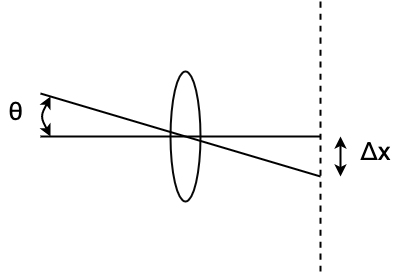
\includegraphics[width=0.8\linewidth]{fig6.png}
 \end{center}
 \caption{光学系}
 \label{fig:6}
\end{figure}

%=============================================================
\newpage
\end{document}

\documentclass[11pt, a4paper,twocolumn]{jarticle}
\usepackage[dvipdfmx]{graphicx}
\usepackage{listings,jlisting}

\begin{document}
%=============================================================
\section{一次元走査光学系の組み立て}
\subsection{目的}
今回の実験では走査状態での光信号の測定を行うための光学系を作成することが目的である.

\subsection{手順}
図\ref{fig:7}のように光学系を構成した.
ステッピングモーター以外の構成は前回の定常状態での光信号の取得での光学系と同じものを使用した.
半導体レーザーからコリメートされた光をステッピングモーターについている反射鏡に入射させることでモーターの制御で入力物体をx軸方向に走査して光信号を検出できるようにした.
なお,この実験では光学系を作成するのみなので結果,考察を省く.


\begin{figure}[ht]
 \begin{center}
  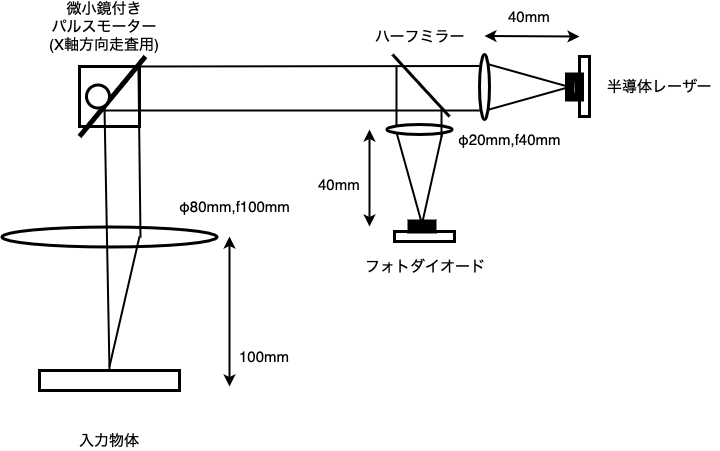
\includegraphics[width=0.8\linewidth]{fig7.png}
 \end{center}
 \caption{一次元走査光学系}
 \label{fig:7}
\end{figure}


%=============================================================
\newpage
\end{document}

\documentclass[11pt, a4paper,twocolumn]{jarticle}
\usepackage[dvipdfmx]{graphicx}
\usepackage{listings,jlisting}

\begin{document}
%=============================================================
\section{走査プログラムの作成と光パターン観察}
\subsection{目的}
今回の実験では前回作成した光学系で光信号を取得するための制御プログラムを作成する.
\subsection{手順}
まず,プログラムを実行すると同時にレーザーが発光し走査が開始され,データをテキストファイルとしてパソコンに書き込んだ後,消光するプログラムを作成した.
なお,実行時にコマンドプロンプトで読み取るデータ点数,サンプリング周波数を設定できるようにした.
次に,ミラーの回転により,入力物体に生成される光スポットの形状がどのように変化するかを観察した.
\subsection{結果}
光スポットの形状は,コリメートされた光が焦点距離100mmの凸レンズの中心付近を通った際には十分集光されたが,凸レンズの中心を外れる程と楕円形に広がって集光されなくなった.

\subsection{考察}
今回実験に用いたレンズは球面平凸レンズだったので,レンズの中心を通る光は十分焦点に集まるがレンズの中心を離れるほど光がぼけていく原因は球面収差によるものであると考えられる.
%=============================================================
\newpage
\end{document}

\documentclass[11pt, a4paper,twocolumn]{jarticle}
\usepackage[dvipdfmx]{graphicx}
\usepackage{listings,jlisting}

\begin{document}
%=============================================================
\section{二値周期パターンの取り込み}
\subsection{目的}
今回の実験は一次元方向にのみ光学濃度が変化する画像データの光信号の取得が目的である.

\subsection{手順}
まず図\ref{fig:8}に示す幅1.2mm,ピッチ2.4mmの二値周期パターン画像を光学系に取り付けた.
その後測定プログラムを実行し,データ点数1000,サンプリング周波数100Hzとして10秒間の測定を行った.

\begin{figure}[ht]
 \begin{center}
  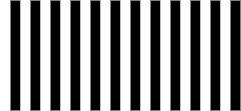
\includegraphics[width=0.8\linewidth]{fig8.png}
 \end{center}
 \caption{二値周期パターン}
 \label{fig:8}
\end{figure}

\subsection{結果}
測定の結果,図\ref{fig:9}のようになった.
周期的に変化する正弦波のような様子が測定できた.

\begin{figure}[ht]
 \begin{center}
  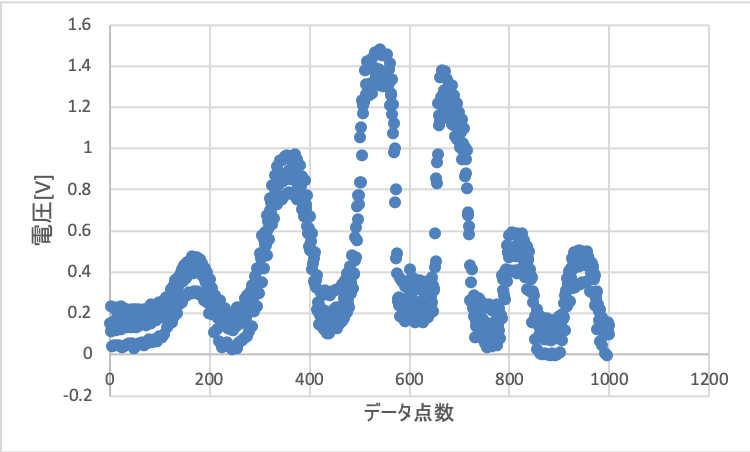
\includegraphics[width=0.8\linewidth]{fig9.png}
 \end{center}
 \caption{二値周期パターンの読み取り}
 \label{fig:9}
\end{figure}


\subsection{考察}
図\ref{fig:9}より4番目,5番目の周期が他の周期に比べて測定電圧が大きくなっているためこの時,コリメートされた光がレンズの中心を通り集光スポットが小さくなっていたと考えられる.
また実験5(ステッピングモーターの動作確認)で求めた1周期あたり$\Delta{x} = 0.0178mm$という値より,今回はエリアシングを起こすことなく正確に測定できたと考えられる.
測定結果がステップ関数のような二値ではなく滑らかな正弦波のようになった原因としては集光した光が入力物体に当たった際に散乱して周りの反射光も取り込んでしまったことや集光スポットが二値の境界線に乗ってしまったことなどが考えられる.
%=============================================================
\newpage
\end{document}

\documentclass[11pt, a4paper,twocolumn]{jarticle}
\usepackage[dvipdfmx]{graphicx}
\usepackage{listings,jlisting}

\begin{document}
%=============================================================
\section{一次元走査光学系の特性評価}
\subsection{目的}
正弦波変調パターンを測定することにより,構成した光学系の特性を評価する.

\subsection{手順}
まず図\ref{fig:10}に示すような正弦波変調パターン画像を入力物体として用いた. \\

\noindent
\textbf{9-1} \\
周期2.0mmパターンのサンプルを用いて表\ref{fig:foo}のように異なる走査ピッチ(サンプリング間隔)で測定を行った. \\

\noindent
\textbf{9-2} \\
データ数2500,サンプリング周波数500に固定し,\ref{fig:foofoo}のようにパターンの周期を変えながら画像データを取得しそのコントラストを求めた. \\

\noindent
\textbf{9-3} \\
物体を光軸と垂直方向にシフトさせ,集光スポットが楕円形になった状態から計測を開始し,2と同様に測定を行った.
この際,データ数2500,サンプリング周波数500に固定し,0.4mm,0.6mmのパターン周期での測定は省略した.

\begin{table}[ht]
\centering
\caption{実験9-1}
\begin{tabular}{c c c}
\hline
 & データ数 & サンプリング周波数[Hz] \\ \hline
9-1-1 & 10000 & 1000 \\
9-1-2 & 5000 & 500 \\
9-1-3 & 1000 & 100 \\
9-1-4 & 100 & 10 \\
9-1-5 & 10 & 1 \\
\end{tabular}
\label{fig:foo}
\end{table}

\begin{table}[ht]
\centering
\caption{実験9-2}
\begin{tabular}{c c}
\hline
 & パターン周期[mm]\\ \hline
9-2-1 & 0.4 \\
9-2-2 & 0.6 \\
9-2-3 & 1.0 \\
9-2-4 & 1.5 \\
9-2-5 & 2.0 \\
9-2-6 & 2.5 \\
\end{tabular}
\label{fig:foofoo}
\end{table}

\begin{figure}[ht]
 \begin{center}
  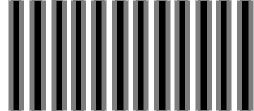
\includegraphics[width=0.8\linewidth]{fig10.png}
 \end{center}
 \caption{正弦波変調パターン}
 \label{fig:10}
\end{figure}

\subsection{結果}
\noindent
\textbf{9-1} \\
測定の結果以下のようなグラフが得られた.

\begin{figure}[ht]
 \begin{center}
  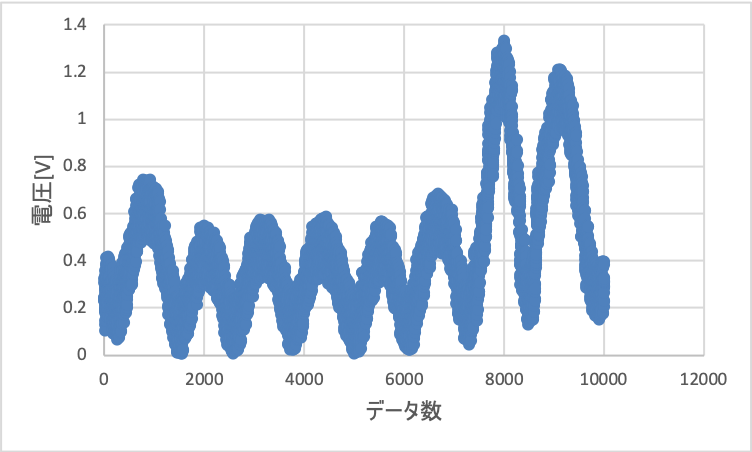
\includegraphics[width=0.8\linewidth]{fig11.png}
 \end{center}
 \caption{9-1-1}
 \label{fig:11}
\end{figure}

\begin{figure}[ht]
 \begin{center}
  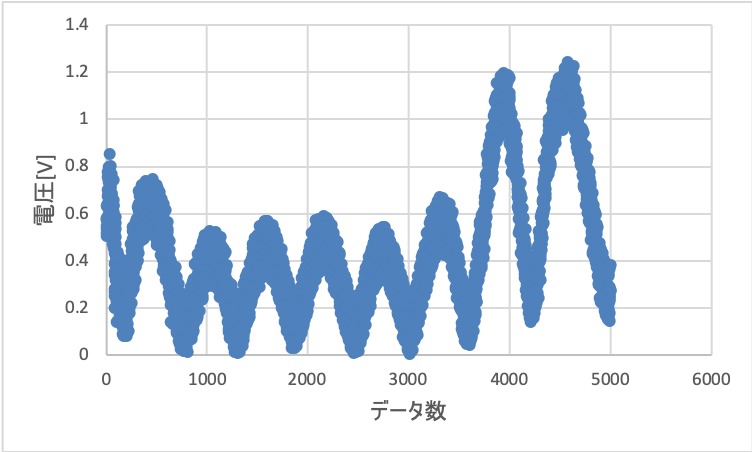
\includegraphics[width=0.8\linewidth]{fig12.png}
 \end{center}
 \caption{9-1-2}
 \label{fig:12}
\end{figure}

\begin{figure}[ht]
 \begin{center}
  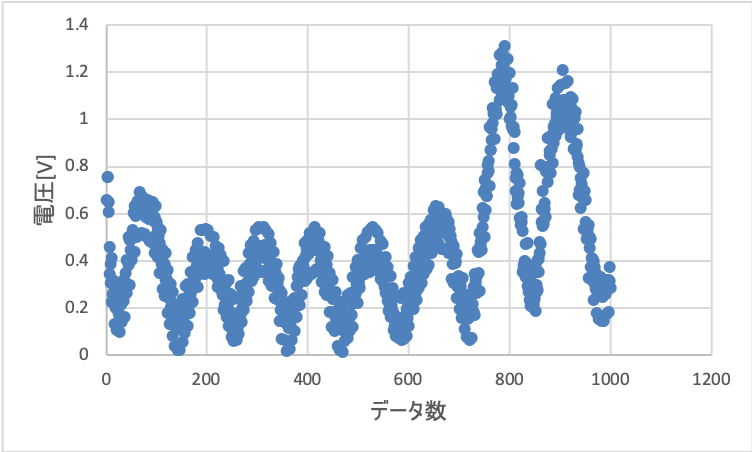
\includegraphics[width=0.8\linewidth]{fig13.png}
 \end{center}
 \caption{9-1-3}
 \label{fig:13}
\end{figure}

\begin{figure}[ht]
 \begin{center}
  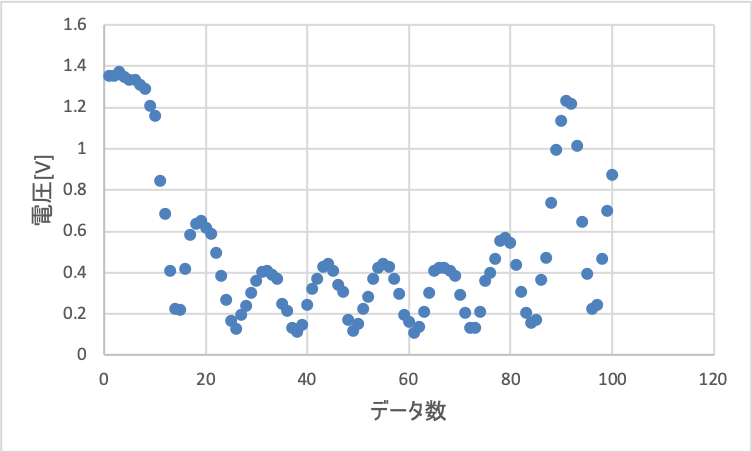
\includegraphics[width=0.8\linewidth]{fig14.png}
 \end{center}
 \caption{9-1-4}
 \label{fig:14}
\end{figure}

\begin{figure}[ht]
 \begin{center}
  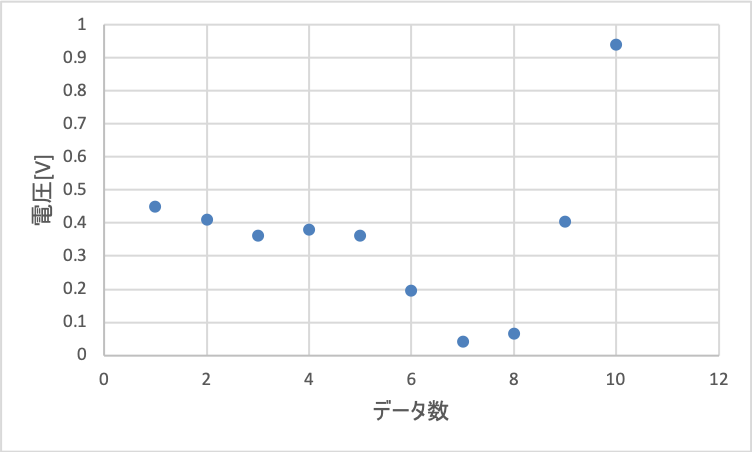
\includegraphics[width=0.8\linewidth]{fig15.png}
 \end{center}
 \caption{9-1-5}
 \label{fig:15}
\end{figure}

\noindent
\textbf{9-2} \\
測定の結果以下のようなグラフが得られた.

\begin{figure}[ht]
 \begin{center}
  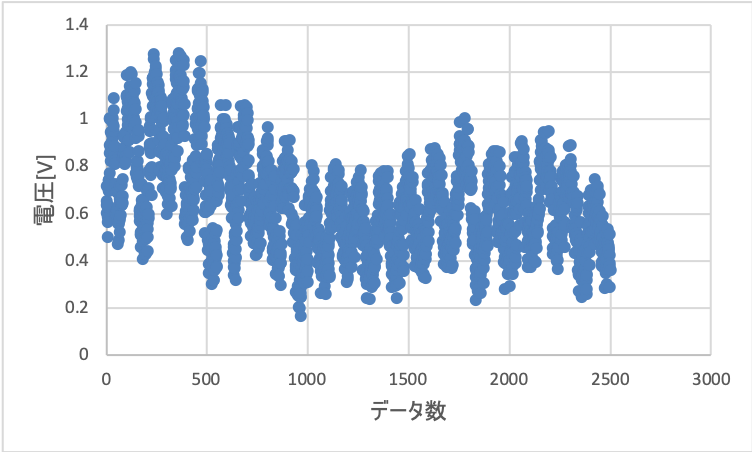
\includegraphics[width=0.8\linewidth]{fig16.png}
 \end{center}
 \caption{9-2-1}
 \label{fig:16}
\end{figure}

\begin{figure}[ht]
 \begin{center}
  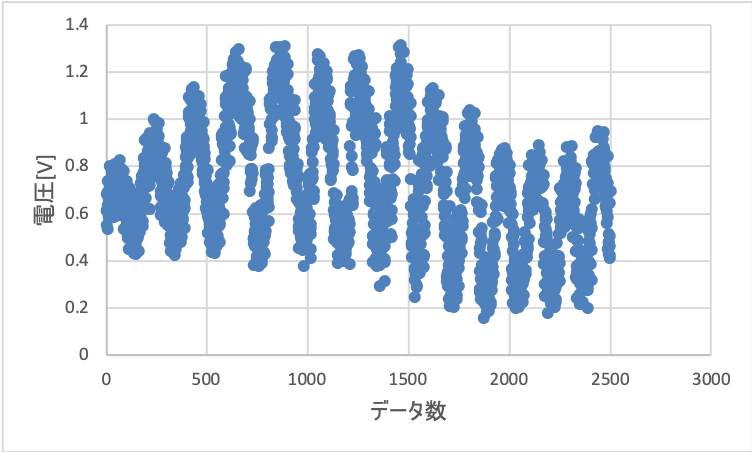
\includegraphics[width=0.8\linewidth]{fig17.png}
 \end{center}
 \caption{9-2-2}
 \label{fig:17}
\end{figure}

\begin{figure}[ht]
 \begin{center}
  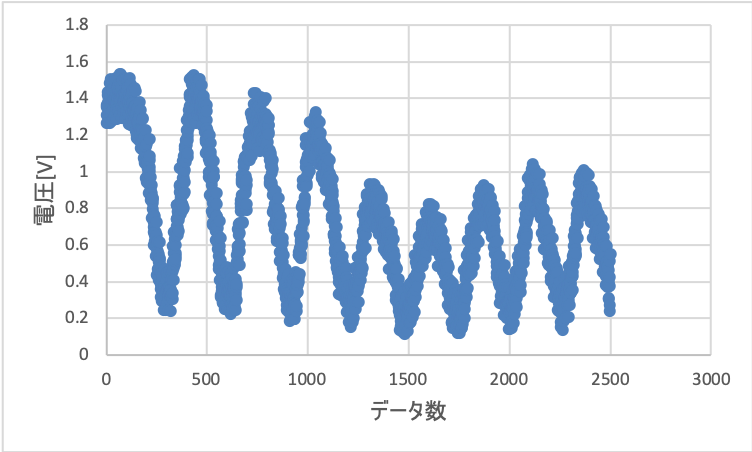
\includegraphics[width=0.8\linewidth]{fig18.png}
 \end{center}
 \caption{9-2-3}
 \label{fig:18}
\end{figure}

\begin{figure}[ht]
 \begin{center}
  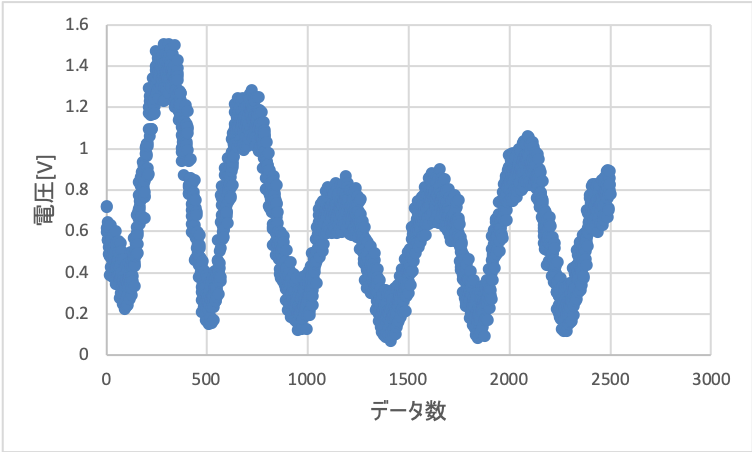
\includegraphics[width=0.8\linewidth]{fig19.png}
 \end{center}
 \caption{9-2-4}
 \label{fig:19}
\end{figure}

\begin{figure}[ht]
 \begin{center}
  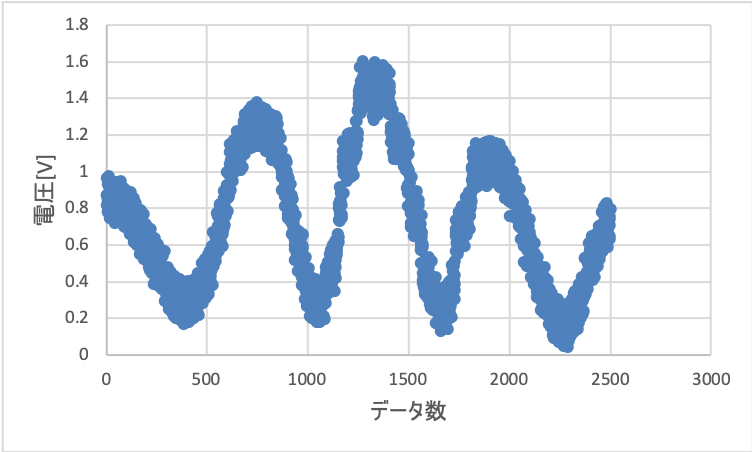
\includegraphics[width=0.8\linewidth]{fig20.png}
 \end{center}
 \caption{9-2-5}
 \label{fig:20}
\end{figure}

\begin{figure}[ht]
 \begin{center}
  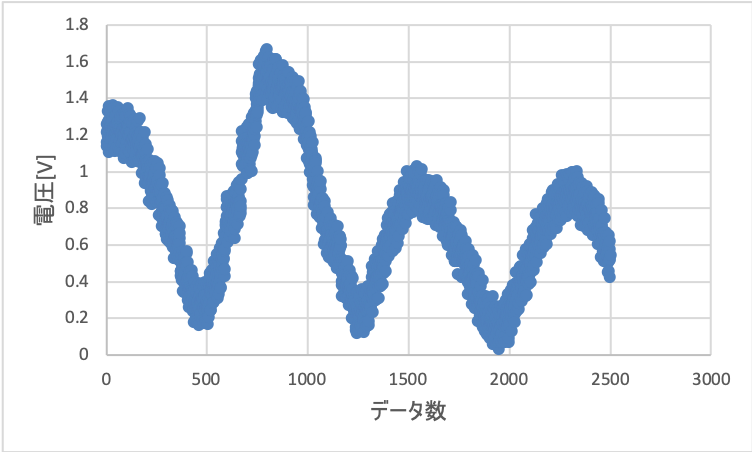
\includegraphics[width=0.8\linewidth]{fig21.png}
 \end{center}
 \caption{9-2-6}
 \label{fig:21}
\end{figure}

\noindent
\textbf{9-3} \\
測定の結果以下のようなグラフが得られた.

\begin{figure}[ht]
 \begin{center}
  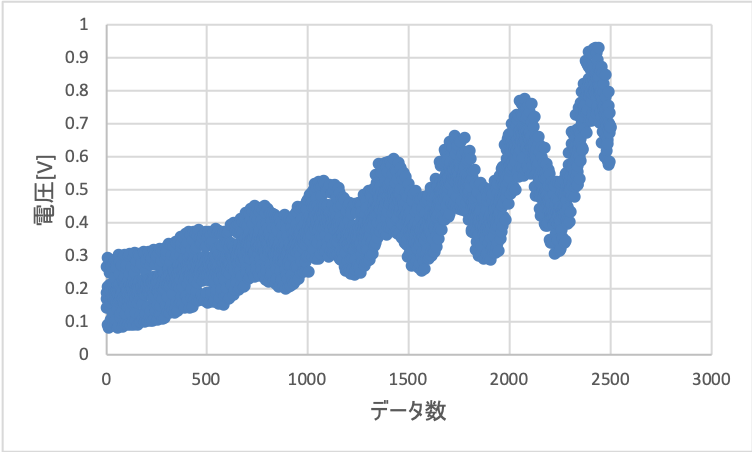
\includegraphics[width=0.8\linewidth]{fig22.png}
 \end{center}
 \caption{9-3-1}
 \label{fig:22}
\end{figure}

\begin{figure}[ht]
 \begin{center}
  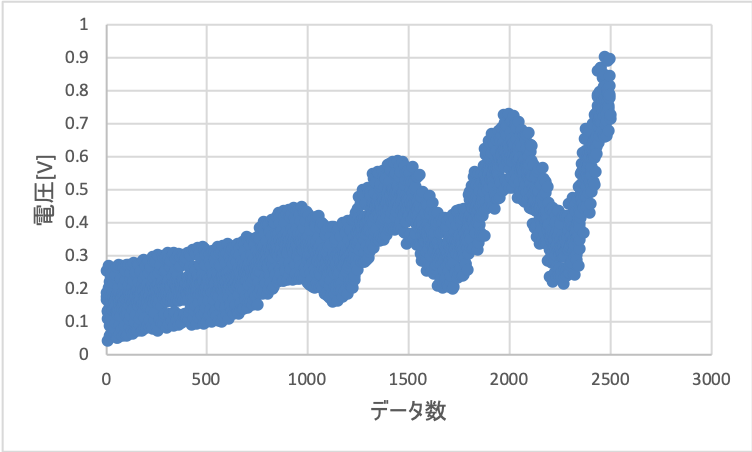
\includegraphics[width=0.8\linewidth]{fig23.png}
 \end{center}
 \caption{9-3-2}
 \label{fig:23}
\end{figure}

\begin{figure}[ht]
 \begin{center}
  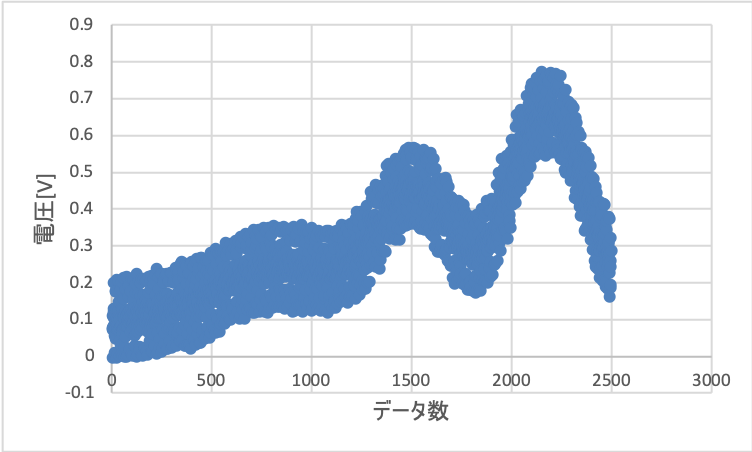
\includegraphics[width=0.8\linewidth]{fig24.png}
 \end{center}
 \caption{9-3-3}
 \label{fig:24}
\end{figure}

\begin{figure}[ht]
 \begin{center}
  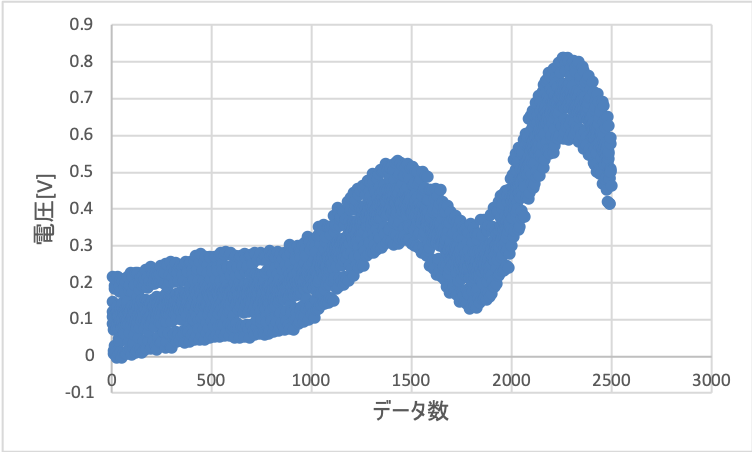
\includegraphics[width=0.8\linewidth]{fig25.png}
 \end{center}
 \caption{9-3-4}
 \label{fig:25}
\end{figure}

\clearpage

\subsection{考察}
まず実験9-1においては図\ref{fig:14}まではパターン周期と同じように測定できている一方で図\ref{fig:15}においては測定対象の周期を正確に読み取れていないため,走査ピッチが大きすぎたことによるエリアシングが起きたと考えられる.
サンプリング定理よりサンプリング周波数はは測定対象のパターン周波数の2倍より多くとっておく必要があると予測される.
実験9-2においては0.2mmのサンプルに対しても正確な測定を行うことができたのでこの光学系の分解能は0.2mm以上であることが予想される.
ここで,集光スポットの半径を求めてみる.
コリメートされた光は楕円形であり長軸1.5mm,短軸1.4mmであるのでDをレーザー直径,lをレーザー波長($l=6.5\times{10^{-6}}mm$),fをレンズの焦点距離として回折限界の式に代入する.

\begin{eqnarray}
    D_0 &=& \frac{4fl}{\pi D} \\
        &=& 59.1\mu m
\end{eqnarray}
以上の結果と実験後においてのスッテッピングモーターの1周期分の移動量$\Delta x = 17.8\mu m$を考慮すると0.06mm周期のパターン周期まで測定可能であると考えることができる.
さらに,この光学系の分解能をさらに上げるためには上の分解能の式よりより波長の短いレーザーを使用する,コリメートする際により直径を大きくする,焦点距離の小さなレンズを使用するなどが考えられる.
さらにステッピングモーターの1周期分の回転角をさらに小さくし,集光する際に球面レンズではなく非球面レンズを用いて球面収差を抑えてで走査範囲を広げることができると考えられる.
%=============================================================
\newpage
\end{document}

%=============================================================
\begin{thebibliography}{9}
  \bibitem{1} 石飛 秀和 他, 「応用物理学実験」
  \bibitem{2} 櫛田 孝司  , 「光物理学」
\end{thebibliography}
%=============================================================
\end{document}
